\section{Алгоритм SIFT}

\textbf{Scale-invariant feature transform} (SIFT) - алгоритм компьютерного зрения для выделения ключевых точек и их дескрипторов. Алгоритм был разработан в Университете Британской Колумбии и опубликован Дэвидом Лоу (\textit{David G. Lowe}) в 1999 году \hyperref[itm:lowe]{[\ref{itm:lowe}]}.

На первом этапе часто производится предварительная обработка изображения в целях улучшения его качества для последующего анализа. Например, на фотографиях с камер возможно появление шумов. Чтобы их устранить используют гауссовское размытие с маленьким радиусом или медианные фильтры.

\subsection{Извлечение ключевых точек}

Основополагающим моментом в нахождении особых точек является построение пирамиды гауссианов (\textbf{Gaussian}) и разностей гауссианов (\textbf{Difference of Gaussian, DoG}). Гауссианом (или изображением, размытым гауссовым фильтром) является изображение:
\begin{equation} \label{eq:1}
    L(x,y,\sigma) = G(x,y,\sigma) * I(x,y)
\end{equation}

В уравнении (\ref{eq:1}): $L$ — значение гауссиана в точке с координатами $(x,y)$, а $\sigma$ — радиус размытия. $G$ — гауссово ядро, $I$ — значение исходного изображения, $*$ — операция свертки.

Разностью гауссианов называют изображение, полученное путем попиксельного вычитания одного гауссина исходного изображения из гауссиана с другим радиусом размытия:
\begin{equation} \label{eq:2}
    D(x,y,\sigma) = (G(x,y,k\sigma)-G(x,y,\sigma)) * I(x,y) = L(x,y,k\sigma) - L(x,y,\sigma)
\end{equation}

Таким образом, с помощью (\ref{eq:1}), мы получаем набор изображений, являющихся исходным изображением взятым в разных масштабах. Извлечение ключевых точке на определённом изображении из этого набора будет гарантировать инвариантность относительно сдвига, поворота и изменения размера изображения.

Как же выбирается нужный масштаб исходного снимка?. Для этого строится пирамида гауссианов (Рисунок \ref{fig:dog1}): весь набор масштабированных изображений разбивается на некоторые участки - октавы и при переходе от одной октавы к другой размеры изображения уменьшаются вдвое. После этого строится пирамида разностей гауссианов, состоящая из разностей соседних изображений в пирамиде гауссианов.

\begin{figure}[h]
    \centering
    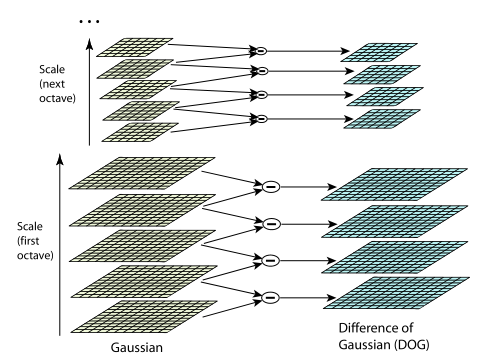
\includegraphics[width=0.6\textwidth]{dog.png}
    \caption{Пирамида гаусианнов}
    \label{fig:dog1}
\end{figure}

После построения пирамиды разностей гауссианов по всем точкам в пирамиде ищутся локальные экстремумы. Если точка больше (меньше) всех своих 26 соседей (Рисунок \ref{fig:dog2}) в пирамиде разностей, то она считается ключевой.

\begin{figure}[h]
    \centering
    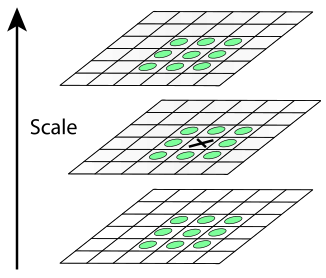
\includegraphics[width=0.5\textwidth]{dog2.png}
    \caption{Локальный экстремум в пирамиде Гауссианов}
    \label{fig:dog2}
\end{figure}

Направление особой точки вычисляется на изображении из пирамиды гауссианов в масштабе, полученном на предыдущем шаге. Ориентация ключевой точки - суммарное направление градиентов точек, находящихся в  $\sigma$-окрестности особой точки. Каждая точка окрестности влияет на итоговое направление. Величина и направление градиента в точке $(x,y)$ вычисляются по формулам (\ref{eq:3}) и (\ref{eq:4}) соответственно.

\begin{equation} \label{eq:3}
    m(x,y)=\sqrt{(L(x+1,y) - L(x-1,y))^2 + (L(x,y+1) - L(x,y-1))^2}
\end{equation}

\begin{equation} \label{eq:4}
    \theta(x,y)=\arctan{\left(\frac{L(x,y+1) - L(x,y-1)}{L(x+1,y) - L(x-1,y)}\right)}
\end{equation}

Таким образом для исходных изображений разных размеров мы получили ключевые точки (и небольшую область возле них) одного и того же размера - это и даёт инвариантность относительно масштабирования. А с помощью ориентации особой точки достигается инвариантность относительно поворота.

\subsection{Извлечение дескрипторов}

Как уже говорилось ранее, дескриптор должен уникально описывать ключевую точку. В общем случае это может быть любой объект, который будет выполнять данные функции: быть удобным для сравнения и являться инвариантным относительно преобразований исходного изображения.

В алгоритме SIFT дескриптор представляется как вектор, содержащий информацию об окрестности ключевой точки. Дескриптор вычисляется на том же гауссиане, на котом получен оптимальный размер особой точки. Для достижения инвариантности относительно поворота изображения перед вычислением всю область ключевой точки поворачивают на угол направления ключевой точки.

\begin{figure}[h]
    \centering
    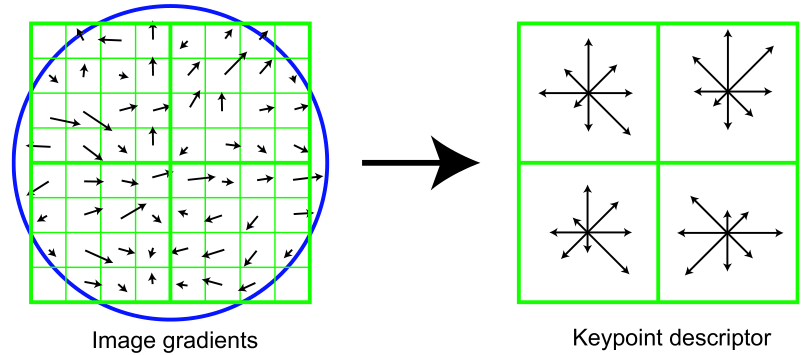
\includegraphics[width=0.8\textwidth]{desc.png}
    \caption{Получение дескриптора}
    \label{fig:desc}
\end{figure}

На Рисунке \ref{fig:desc} показана окрестность ключевой точки (слева) и построенный для неё дескриптор, состоящий из гистограмм (справа). Стрелочками в центре каждого пикселя в $\sigma$-окрестности обозначен градиент этого пикселя. Как видно на правой стороне изображения, дескриптор имеет размерность 2x2x8 (количество регионов по горизонтали, количество регионов по вертикали, количество компонент гистограммы этих регионов). Гистограмма для каждого региона является суммарным значением градиентов пикселей, входящих в $\sigma$-окрестность ($8$ штук).

Все полученные гистограммы и составляют итоговый дескриптор ключевой точки. В конце дескриптор нормализуется - все компоненты делятся на максимальное значение - в итоге каждая компонента находится в диапазоне $[0,1]$. Далее всем компонентам, значение которых больше $0.2$, присваивается значение $0.2$, а после этого дескриптор нормализуется ещё раз.

Как говорилось ранее, размер дескриптора равен 2x2x8 = $32$ компоненты, но на практике больше распространены и активнее используются дескрипторы размерности $128$ компонент (4x4x8).
